% !TeX root = Bericht.tex
% !TeX spellcheck = de_DE 
\section{Appendix}\label{sec:appendix}

\begin{figure}[H]
	\centering
	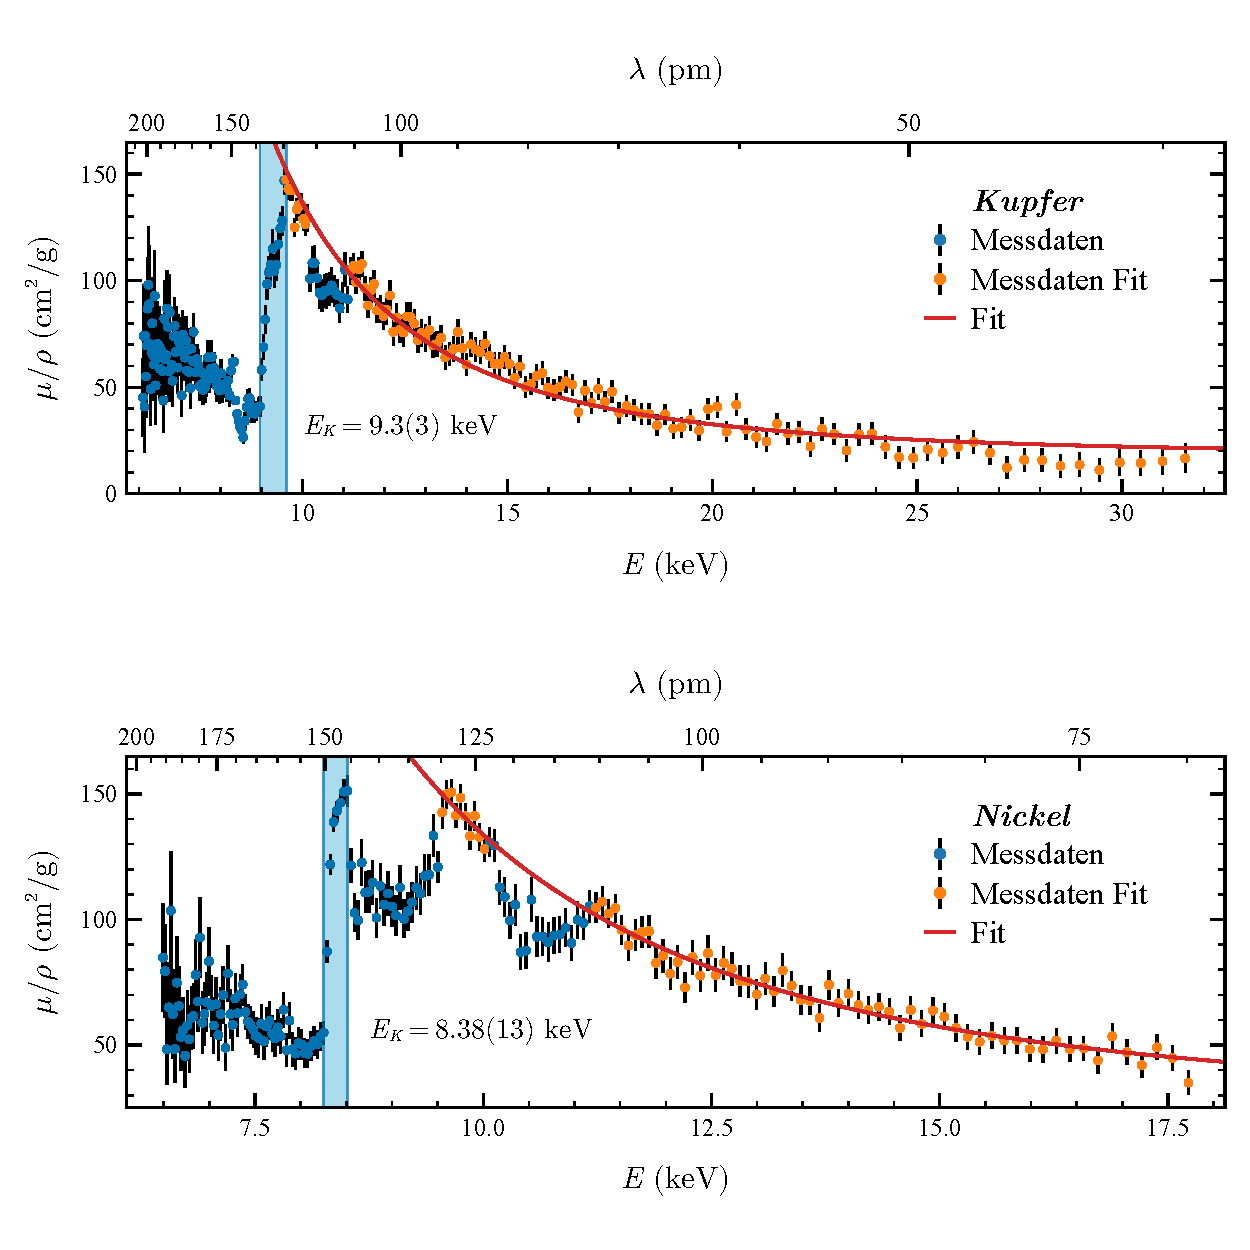
\includegraphics[width=\textwidth]{Ex4_3}
	\caption{Der Massenabsorptionskoeffizient \( \mu/\rho \) ist für Kupfer (oben) und Nickel (unten) auf die Energie sowie Wellenlänge aufgetragen. Ab einer bestimmten Energie \( E_{ion} \) ändert sich das Verhalten sprunghaft. Danach lässt sich eine \( 1/E^3 \) Abhängigkeit beobachten, was durch eine Fitfunktion in Rot angedeutet wird. Substrukturen wurden aus dem Fit ausgenommen.}
	\label{fig:plot3}
\end{figure}

\begin{figure}[H]
	\centering
	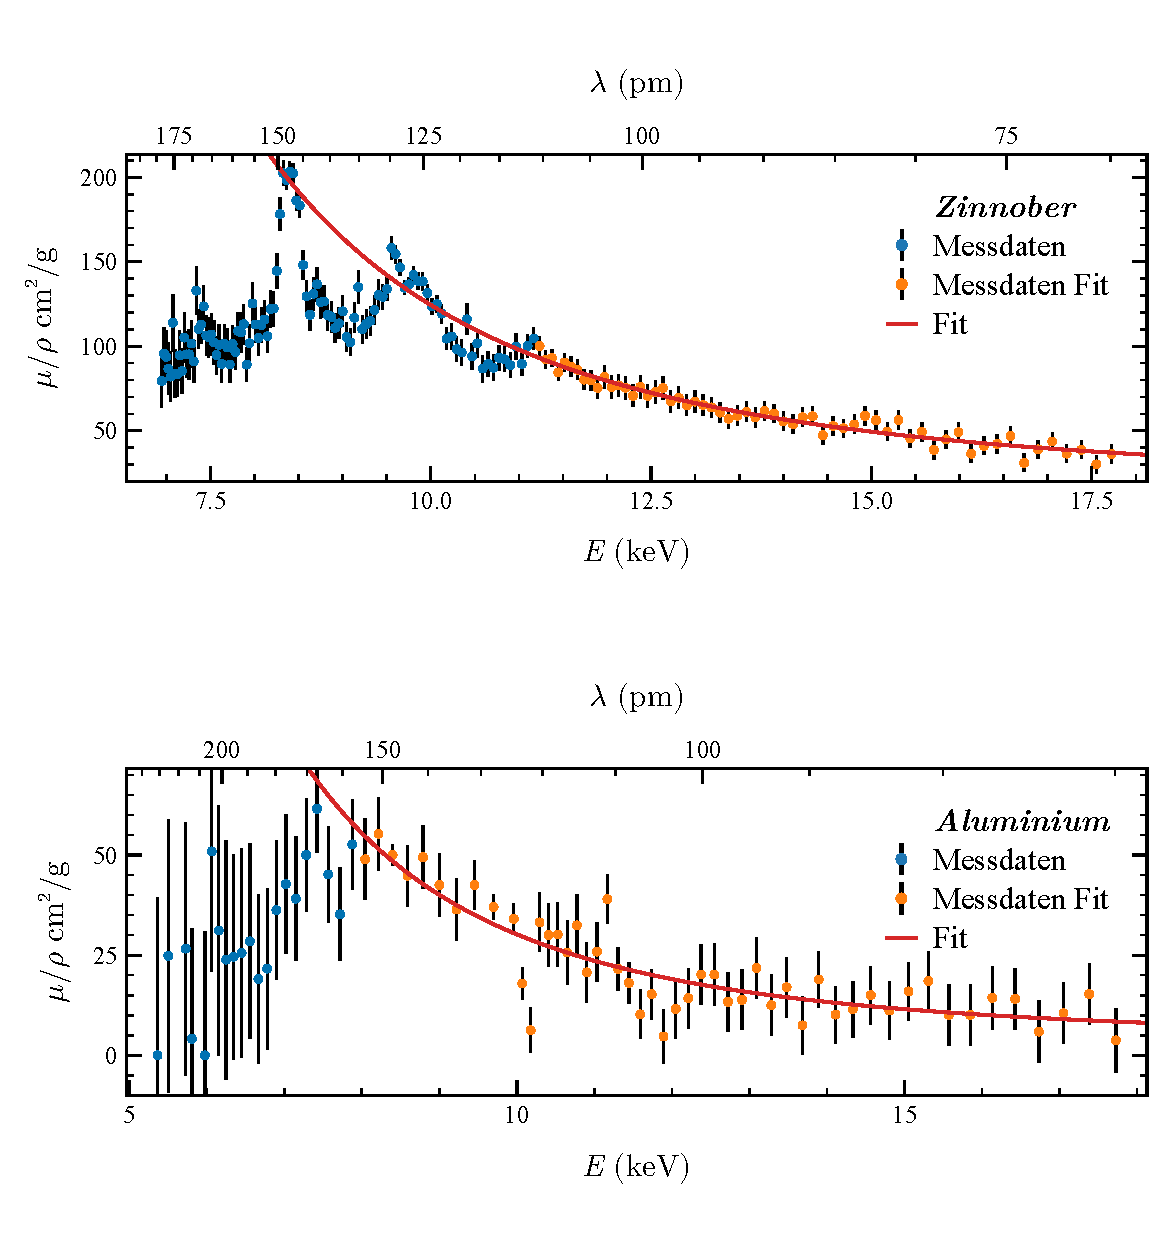
\includegraphics[width=\textwidth]{Ex4_2}
	\caption{Der Massenabsorptionskoeffizient \( \mu/\rho \) ist für Zinnober (oben) und Aluminium (unten) auf die Energie sowie Wellenlänge aufgetragen. Gegen höhere Energien lässt sich eine \( 1/E^3 \) Abhängigkeit beobachten, was durch eine Fitfunktion in Rot angedeutet wird. Substrukturen wurden aus dem Fit ausgenommen.}
	\label{fig:plot3}
\end{figure}

\begin{figure}[H]
	\centering
	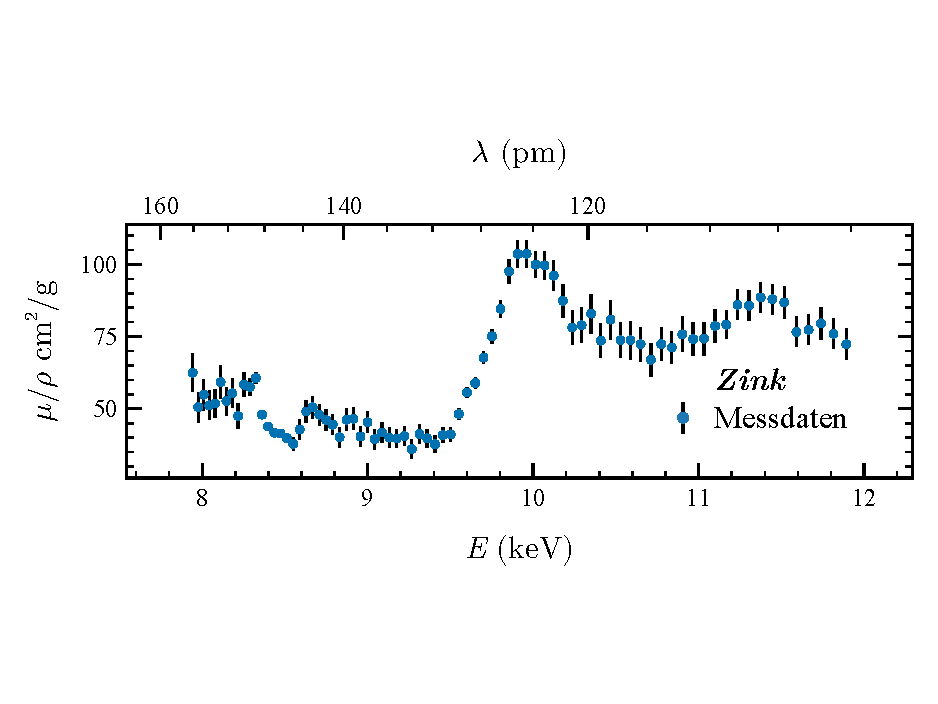
\includegraphics[width=\textwidth]{Ex4_Zn}
	\caption{Der Massenabsorptionskoeffizient \( \mu/\rho \) ist für Zink auf die Energie sowie Wellenlänge aufgetragen.}
	\label{fig:plot3}
\end{figure}